% PLEASE USE THIS FILE AS A TEMPLATE
% Check file iosart2x.tex for more examples

% add. options: [seceqn,secthm,crcready]
\documentclass[sw]{iosart2x}
\usepackage{todonotes}
\usepackage{cleveref}
\usepackage{csquotes}
\usepackage{aurl}
\usepackage{booktabs}
\usepackage{tabulary}
%\usepackage{dcolumn}

%%%%%%%%%%% Put your definitions here
\newcommand{\aw}{AnthroWorks3D}
\daurl{anno}{https://annosaxfdm.de/ontology/}

%%%%%%%%%%% End of definitions

\pubyear{2023}
\volume{0}
\firstpage{1}
\lastpage{1}

\begin{document}

\begin{frontmatter}

%\pretitle{}
\title{The Anthropological Notation Ontology (ANNO): A core ontology for annotating human bones and deriving phenotypes}
\runtitle{Anthropological Notation Ontology}
%\subtitle{}

% For one author:
%\author{\inits{N.}\fnms{Name1} \snm{Surname1}\ead[label=e1]{first@somewhere.com}}
%\address{Department first, \orgname{University or Company name},
%Abbreviate US states, \cny{Country}\printead[presep={\\}]{e1}}
% Höffner, Heuschkel, Schmiedel, Penne, Fritzsch, Ludwig, Mohaupt, Labudde, Uciteli
% TODO: overleaf
% Two or more authors:
\begin{aug}
\author[B]{\inits{M.}\fnms{Marie} \snm{Heuschkel}\ead[label=e2]{marie.heuschkel@hs-mittweida.de}}
\author[A]{\inits{K.}\fnms{Konrad} \snm{Höffner}\ead[label=e1]{konrad.hoeffner@uni-leipzig.de}%
\thanks{Corresponding author. \printead{e1}.}
\thanks{Equal contribution.}%how to show this for the first 3?
}
\author[B]{\inits{F.}\fnms{Fabian} \snm{Schmiedel}\ead[label=e3]{fabian.schmiedel@hs-mittweida.de}}
\author[B]{\inits{L.}\fnms{Laura} \snm{Penne}\ead[label=e4]{laura.penne@hs-mittweida.de}}
\author[B]{\inits{H. T.}\fnms{Hanjo Tim} \snm{Fritzsch}\ead[label=e5]{fritzsc2@hs-mittweida.de}}
\author[B]{\inits{N.}\fnms{Niklas} \snm{de Sousa Norte}\ead[label=e6]{niklas.desousanorte@hs-mittweida.de}}
\author[B]{\inits{A.}\fnms{Andrea} \snm{Ferencová}\ead[label=e7]{andrea.ferencova@hs-mittweida.de}}
\author[B]{\inits{A.}\fnms{Andy} \snm{Ludwig}\ead[label=e8]{andy.ludwig@hs-mittweida.de}}% ist jetzt beim Fraunhofer, möchte aber weiter so gelistet werden
\author[B]{\inits{M.}\fnms{Marleen} \snm{Mohaupt}\ead[label=e9]{kreuzer@hs-mittweida.de}}
\author[B]{\inits{D.}\fnms{Dirk} \snm{Labudde}\ead[label=e10]{dirk.labudde@hs-mittweida.de }}
\author[A]{\inits{A.}\fnms{Alexandr} \snm{Uciteli}\ead[label=e11]{alexander.uciteli@imise.uni-leipzig.de}}
%\author[B]{\inits{}\fnms{} \snm{}\ead[label=e9]{}}
\address[A]{Institute for Medical Informatics, Statistics and Epidemiology (IMISE), \orgname{Leipzig University},
Saxony, \cny{Germany}\printead[presep={\\}]{e1,e11}}
\address[B]{\orgname{Hochschule Mittweida},
Saxony, \cny{Germany}\printead[presep={\\}]{e2,e3,e4,e5,e6,e7,e8,e9,e10}}
\end{aug}

%\begin{review}{editor}
%\reviewer{\fnms{First} \snm{Editor}\address{\orgname{University or Company name}, \cny{Country}}}
%\reviewer{\fnms{Second} \snm{Editor}\address{\orgname{First University or Company name}, \cny{Country}
%  and \orgname{Second University or Company name}, \cny{Country}}}
%\end{review}
%\begin{review}{solicited}
%\reviewer{\fnms{First} \snm{Solicited reviewer}\address{\orgname{University or Company name}, \cny{Country}}}
%\reviewer{\snm{anonymous reviewer}}
%\end{review}
%\begin{review}{open}
%\reviewer{\fnms{First} \snm{Open Reviewer}\address{\orgname{University or Company name}, \cny{Country}}}
%\end{review}

\begin{abstract}
The Anthropological Notation Ontology (ANNO) allows the systematic, standardised classification of recovered bone finds into the skeletal system, the description of the skeletal pieces, and the definition of functions for the derivation of different phenotypes of humans in forensic and historical anthropology.
ANNO consists of two components:
ANNOdc, a domain-core ontology providing core entities such as basic anatomical categories, and ANNOds, a domain-specific ontology used for annotating structures of the human skeleton.
ANNO is integrated into AnthroWorks3D (AW3D), an application for the creation and analysis of 3D-models of human skeletal remains.
The integration is based on the three-ontology method with the General Formal Ontology as the top level ontology, ANNOdc as the task ontology and ANNOds as the domain ontology.
Thus, AnthroWorks3D only needs to implement access to the entities (classes and properties) of the task ontology, whereas the entities of the corresponding domain ontology are processed dynamically.
ANNO supports the analysis of skeletal and bone finds in forensic and historical anthropology, facilitating the standardisation of data annotation and ensuring accurate preservation of information for posterity.
\end{abstract}

\begin{keyword}
\kwd{Ontology}
\kwd{Ontology development}
\kwd{Anthropology}
\end{keyword}

\end{frontmatter}

%%%%%%%%%%% The article body starts:
% TODO notes from meeting, einarbeiten:
% 3 Teile Kernmodule mit Use Cases, weitere Komponenten durch Community


\section{Introduction}\label{sec:introduction}

Data from historical and prehistoric anthropology~\citep{prehistoricanthropology}, as well as modern forensic science, allows for a comprehensive understanding of deceased individuals from different time periods, ranging from their identity and health status to aspects of their behaviour, lifestyle, culture and even concerning the circumstances of their death~\citep{spurensuche}.
For example, anthropological methods can be used to determine individual properties (phenotypes) such as their sex, age, height and ancestry and further individualising traits.

Digitalisation offers several advantages to anthropology, including remote work, without the effects of wear and tear on the physical skeletal specimens.
Current problems of access can be resolved, as examinations can be conducted even if the skeletal material from individuals or collectives are not present at the institution or may have already been reburied, which facilitates interdisciplinary collaborative research.
Moreover it allows for linking data of different study samples across geographical boundaries.
Data sets consolidated this way and formalised through the Anthropological Notation Ontology (ANNO) presented here allow for efficient data analysis techniques, such as data and text mining that promote deeper insights.

Apart from contextual information, most informative clues can be found directly on the bone.
Anthropologists use human anatomy, specifically the skeletal system and further tissues of the musculoskeletal system, to classify and describe and thus document bones, anatomical structures and diagnostic features within the overall framework of the skeleton in a comprehensive and transparent fashion.

Applying the same principles used for mapping the Earth’s surface \enquote{terrain}, it is possible to create a detailed map of the human body containing visible anatomical surface structures as well as artificial objects such as measurement points or content-related or methodologically based classifications and boundaries~\citep{topo}. ANNO represents such a map by providing an ontology for accurate and exhaustive definitions that allow to unequivocally locate these, ensure their easy retrieval and furthermore serve as a basis for the objective examination, for instance in the form of measurements.


ANNO consists of two components: ANNOdc, a domain-core ontology providing core entities such as basic anatomical concepts and classifications, and ANNOds, a domain-specific ontology employed for annotating human skeletal structures. In its current version, the ontology  refers to standardised normal adult anatomy, excluding developmental aspects, variations, pathologies and other related factors. ANNO is integrated into AnthroWorks3D (AW3D), an application for generating and analysing 3D-models of human skeletal remains. 


\section{Related Work}

There are various reference materials for the description of anatomical structures, ranging from anatomical atlases to nomenclatures.
The latter aim for an established standardised naming and systematisation.
There are currently two prominent ontologies in the field of general anatomy:

The Terminologia anatomica~\citep{ta2} (TA) is a hierarchy of anatomical structure concepts for the entire human body.
For historical reasons, it uses a terminology consisting of Latin and originally Greek, which was later latinised.
For each anatomical structure, the TA provides the \enquote{preferred}, i.e. standard, Latin term and its English equivalent as well as an individual identification number.
In some cases, Latin and English synonyms are also included, e.g. \emph{malar bone} is an English synonym of the Latin preferred term \emph{Os zygomaticum} and its English equivalent \emph{zygomatic bone}.
The identification number is crucial, as certain landmarks are mostly listed without bone affiliation, resulting in multiple occurrences. %(s. Bone Part)
For instance, the \emph{processus zygomaticus} can be found both at the \emph{os frontale} and the \emph{os temporale}.
Eponyms are terms derived from proper nouns such as the name of a person, place or thing, and they are considered a type of synonyms since they stand for the same anatomical structure.
For example, \emph{ossa digitorum manus / pedis} (engl. \emph{phalanges of the hand / foot}) are the small bones of the fingers and toes and are also denoted as \emph{phalanges manus / pedis} which are named after the Greek word \emph{phalanx} for a dense rectangular infantry formation.
In addition to the outdated print edition~\citep{ta1998}, an extended second edition (TA2) is available online~\citep{ta2}.
Furthermore, there is a commercially available independent companion print publication with German~\citep{anatomylexicon}, English~\citep{pocketatlas} and Spanish~\citep{taspanish} editions of which at least the German edition is regularly updated.
This book contains textual and visual descriptions, whereby anatomical structures are indicated through lines on the illustrations.

The \emph{Foundational Model of Anatomy} (FMA)~\citep{fma} ontology represents the physical organisation of human anatomy by mapping relations to one another.
It allows the knowledge it contains to be represented in a way that is humanly comprehensible and machine-interpretable.
The FMA uses the Basic Formal Ontology (BFO) as its top level ontology.
Corresponding to its relational nature, new higher level concepts are introduced and used for reorganising the actual anatomical structures diverging from the TA’s hierarchical structure.
Thus, in 90\,\% of the cases this lead to new creations of anatomical concepts~\citep{anatomicalterms} whereas only 1\,\% contain textual definitions~\citep{uberon}.

We manually created links to FMA.
Wikidata provides unofficial links between the FMA and TA2 which we use to link to TA2.

\subsection{Problems and Research Gaps}

There are several issues and research gaps when it comes to naming and defining anatomical concepts and instances that neither current ontologies nor reference literature---general or subject-specific---can address adequately.

The primary issue lies in the absence of standardisation.
While both the TA and FMA have been proposed as a means of standardising terminology, they haven't garnered sufficient acceptance to facilitate the adoption of a unified and consistent body of work to establish standardisation in actual practice~\citep{frequencyta,doestamatter,athighlights}.
Instead, the usage of terminology is as fluent as any other language, depending on its socio-cultural environment, such as schools or language areas~\citep{doestamatter,atthennow,atinfo,frequencyta,atcompare}.
Thus, the usage of English designations is preferred in the Anglo-American sphere while Latin terms are commonly used in German-speaking areas~\citep{anatomycontribution,anatomylexicon,reforminganatomical}.
As a consequence there are at times various translations for the same anatomical terms~\citep{naminggame}.
Yet, knowledge of Latin is generally declining.
With the terms hence becoming more abstract to the people using them, there is also a common prevalence for spelling divergences or grammar mistakes~\citep{ta17,anatomylexicon,athighlights,diphthongs}.
Moreover, in textual descriptions latin and the native language are commonly used interchangeably for stylistic purposes.
For instance, \cite{anatomylexicon} uses the German terms of the bones in the explanation of sutures.
Meanwhile, the existing terminology is not flexible enough for language-like usage as, for example, there is an inconsistent use of singular and plural forms or gaps in lateralized landmarks.

Anatomical terms, unless historically evolved, typically describe the location, affiliation or function of a concept or structure~\citep{reforminganatomical}.
However, this naming convention is often inconsistent and non-intuitive.
An example, showing the variability in illustrative descriptions are the Tuberculum articulare of the Processus zygomaticus, which in \cite{anatomie} is described as saddle-shaped although it is not called \emph{sella}, the Latin name for saddle.
It is moreover worth pointing out that not every anatomical structures contributing to an articulation in some way, automatically carry the term articular with them, such as the Caput mandibulae, which connects the Mandibula to the rest of the Cranium.
The Tuber frontale, which serves as an indicator for sex in anthropology, is listed as an eminentia in the TA~\citep{ta2}.
Likewise, he Protuberantia mentale is referred to as Eminentia mentale in a widely-used anthropological method that is also used for sex determination.
As can be seen, the incentive for synonyms is high.
However, the current resources fail to provide comprehensive lists of synonyms in use.
This in turn may lead to misattribution, as is the case for example, in the FMA the entry with the \emph{preferred name} \enquote{External acoustic aperture} and \emph{non-English equivalent} \enquote{Porus acusticus externus} (FMA ID: 61301) lists external acoustic meatus (Meatus acusticus externus in Latin) as a synonym.
However, it is not the same, rather the Porus is---as its English name indicates---the opening to the meatus~\citep{anatomylexicon}.
%Furthermore, terms oftentimes lack clear affiliation to the bone to which they belong.
%When considering the whole skeleton, these terms consequently occur multiple times, causing ambiguity.
Occasionally, there are discrepancies and inconsistencies found in the definitions of individual anatomical structures.
For instance, the position of the Corpus ossis pubis varies across different sources~\citep{anatomylexicon,prometheus,allgemeineanatomie,dualereiheanatomie,anatomiedesmenschen}.

%In addition, the ontologies are only inadequately (TA for the last time in 2013, FMA in 2020) updated and do not undergo continuous synchronisation.%add source for that? 11 and 12 in table but no paper.
Another issue is that neither FMA nor TA are tailored to fit the requirements of anthropology or any other specialised field~\citep{fma}.
For example, articular surfaces of the individual bones are relevant anthropologically, yet not all articular surfaces (e.g. on the Ossa carpi or Ossa metatarsi) are defined in the TA or FMA, resulting in further gaps.
A similar situation exists with respect to osteometric measurements.
Established and to some extent standardised osteometric measurement points are only found on the cranium and mandible~\citep{wesenanthropologie}.
 However, since there are measurement distances on all bones, the respective start and end points must also be defined.
Last but not least, both ontologies suffer from a lack of consideration given to anatomical variants~\citep{anatomycontribution}.
Moreover, different disciplines require a different level of detail, which is why nose surgery works with anatomical terms of very detailed anatomical structures~\citep{graysanatomy},
which to the greater part are not found in the FMA or the TA that primarily aim for the standardisation of general (clinical) anatomy~\citep{fma}.
A work of dental anthropology even split the aforementioned Tuberculum articulare (Articular tubercle) in two structures, naming the other \enquote{articular eminence}~\citep{dentalanthropology}.
%Often exchange between these specific fields and general anatomy hardly takes place.
However, there is limited interdisciplinary coordination between the individual disciplines and general anatomy.

Furthermore, anatomical resources often lack adequate visual representation of anatomical structures.
The labelling is often selective, varies by source and mostly relies on arrows for local designation.
However, since they are multi-dimensional structures, it is essential to provide a marker over the entire landmark and delineate it accurately.
The latter also requires a clear textual definition.
Unfortunately, there are currently no equivalent standardised definitions for skeletal anatomy, meanwhile anatomical resources only provide sparse information on this topic.

To adress these issues, it is necessary to develop unified, textual, visual, and detailed descriptive definitions for anatomical concepts and instances.
These definitions should be presented within an easily understandable ontology.

%\url{https://bioportal.bioontology.org/ontologies/FMA}

\section{Ontological Architecture}\label{sec:architecture}

The ontological architecture of ANNO consists of three interrelated layers representing by a top-level ontology, a domain-core ontology and a domain-specific ontology:

\begin{enumerate}
\item We use the General Formal Ontology (GFO)~\citep{gfo} as top-level ontology of ANNO.
In the current paper, we refer especially to the categories \enquote{Material object}, \enquote{Attributive}, \enquote{Relator} as well as the spatial entities of GFO (\cref{sec:core}, \cref{fig:gfo})

\item ANNOdc (\cref{sec:core}, \cref{fig:core}) is a domain-core (dc) ontology to provide the core entities of a domain.
This includes general anatomical categories (Bone and Tooth), a category for describing their characteristics (Anatomical property), anatomical spatial entities (Anatomical space, surface, line and point) as well as the category \emph{Phenotype} to model the rules for determining human phenotypes.
ANNOdc is embedded in the GFO, i.e. the ANNOdc classes are subclasses of GFO classes.

\item ANNOds (\cref{sec:domain}) is a domain-specific (ds) ontology for describing domain-specific entities to be used for annotating the parts of the human skeleton.
These are bones, teeth, their parts and compounds, such as \emph{mandible}, \emph{Mental protuberance} or the facial skeleton.
It is also used for modelling their properties and relations, such as the distance between Mentale dexterum and Mentale sinistrum, needed to derive human phenotypes like sex or height.
ANNOds is embedded in ANNOdc.
\end{enumerate}

% take care to prevent the problems noted by reviewer 1 in https://semantic-web-journal.net/content/modelling-digital-health-data-examode-ontology-histopathology
% TODO: ontology language, expressivity
% TODO: reuse of ontological entities
% TODO: clear validation mechanism
% TODO: top-level ontology?

\section{Description and Foundation of ANNOdc}\label{sec:core}
The core ontology development occurs in close collaboration between ontologists and anthropologists.
The objective is twofold: to adequately represent the most basic anatomical and anthropological entities and to keep the ontology relatively simple and compact.
This approach ensures that domain experts can easily handle the ontology and efficiently integrate it into the \aw{} software.

% Definition/Beschreibung der Kern-Konzepte/Module und -Relationen mit Beispielen, GFO-Einbettung
\begin{figure}[h]
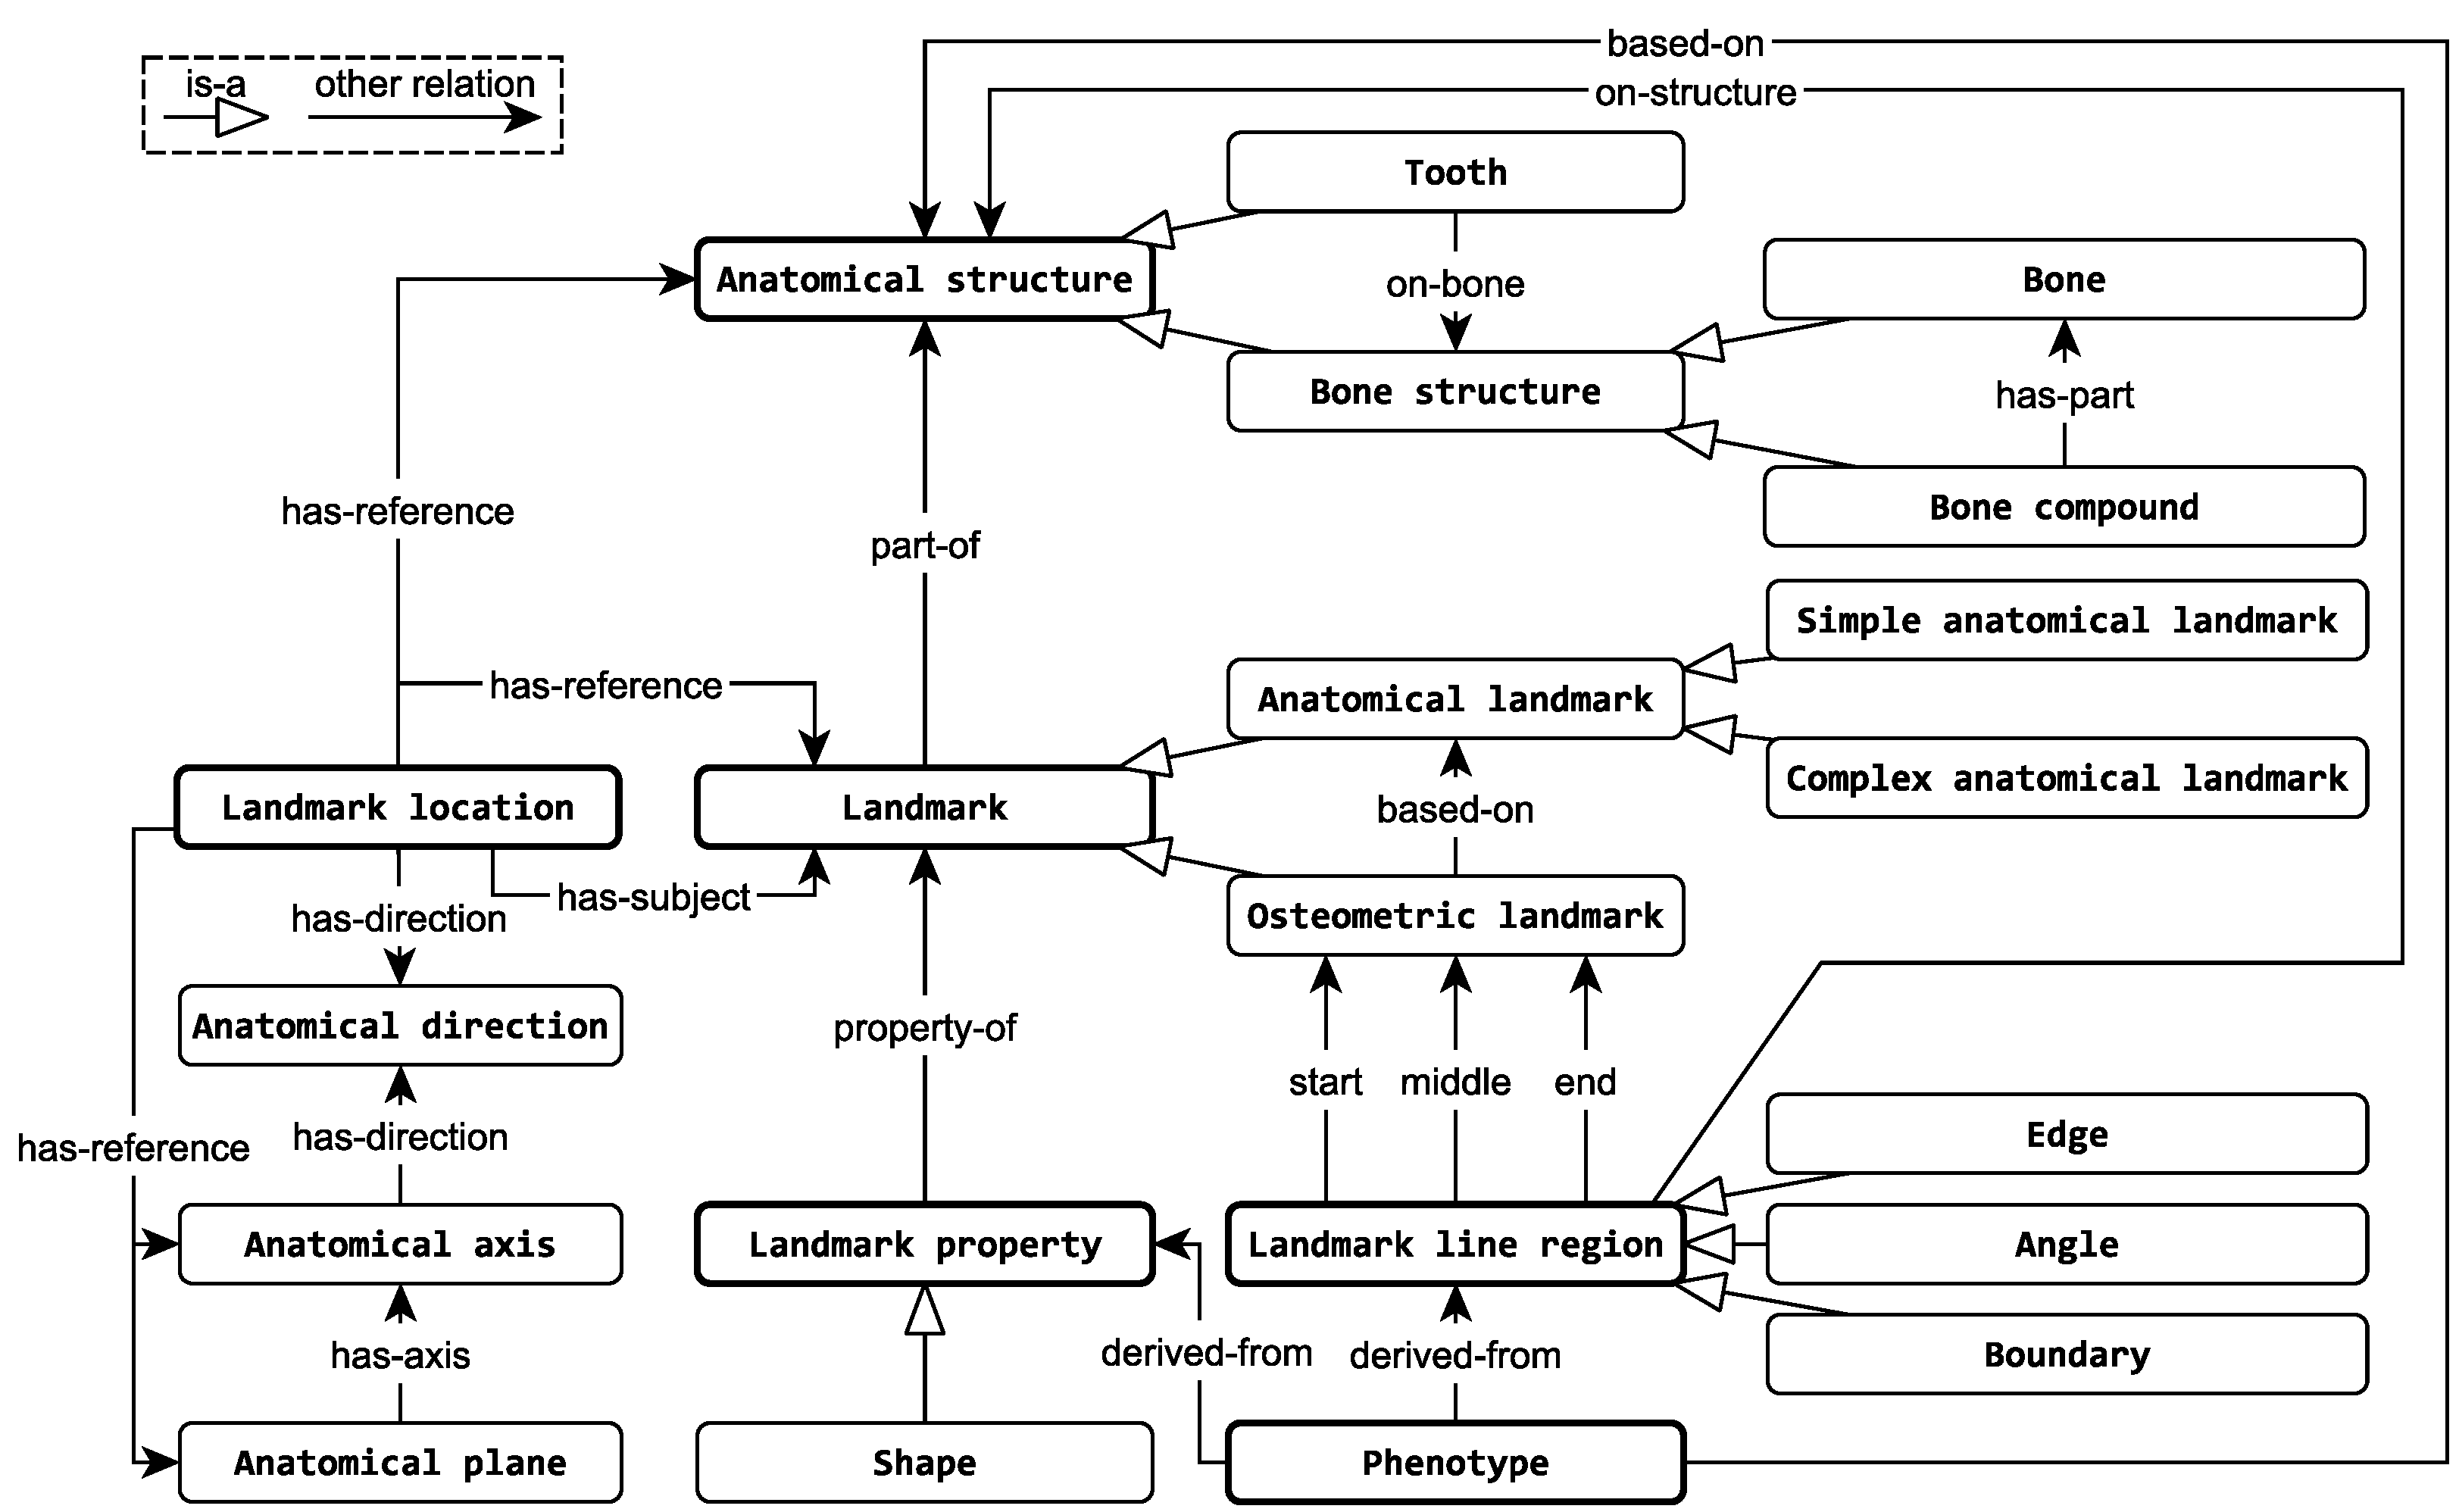
\includegraphics[width=\textwidth]{img/core.pdf}
\caption{ANNOdc ontology}\label{fig:core}
\end{figure}

\begin{table}[htbp]
  \centering
  \caption{Table Title}
  \begin{tabulary}{\textwidth}{lLLl}
    \toprule
	ANNOdc class					&Examples				&FMA equivalent / ID						&GFO superclass	\\
	\midrule
	Anatomical entity			&						&Physical anatomical entity fma61775\\
	Anatomical structure		&						&Material anatomical entity	fma67165		&Material object\\							
	Spatial anatomical entity	&						&immaterial anatomical entity fma:fma67112	&Space entity\\
	Anatomical space			&						&											&Space region\\
	Anatomical surface			&Median Plane			&Anatomical surface fma24137				&Surface region\\
	Anatomical line				&Mandibular Angle (ppam dexter-go dexter-piam dexter), Sagittal Axis&Anatomical line fma9657	&Line region\\
	Anatomical point			&Gonion					&Anatomical point							&Point region\\
	Anatomical plane			&Median Plane			&Anatomical plane fma242982\\
	Anatomical axis		 		&Sagittal Axis\\
	Skeleton					&						&Skeleton fma:fma23875\\
	Bone structure\\
	Bone						&Mandibula				&Bone organ fma:fma5018\\
	
	Bone part					&Protuberantia mentalis	&Related to Segment of bone organ fma:fma281808, Zone of bone organ fma:fma10483\\
	Bone compound				&Cranium				&Comparable to union of Skeletal system fma:fma23881 and subdivision of skeletal system fma:fma85544\\
	Tooth structure				&Dentes Permanentes		&Permanent teeth (fma:fma75152; TA2ID:913)\\
	Tooth						&Dens caninus			&Tooth fma:fma12516\\
	Tooth part					&Cuspis dentis			&fma:fma56481; TA2ID:925\\
	Phenotype					&Height, Sex			&											&Attributive\\							
	Anatomical Property			&Shape (Degree of morphological expression)	&Anatomical relation, e.g., Has\_shape relation	&Attributive\\
	Relative anatomical location&superior, lateral, medial, posterior	&Anatomical qualitative coordinate	&Relator\\
\bottomrule
\end{tabulary}
\end{table}

\begin{figure}[h]
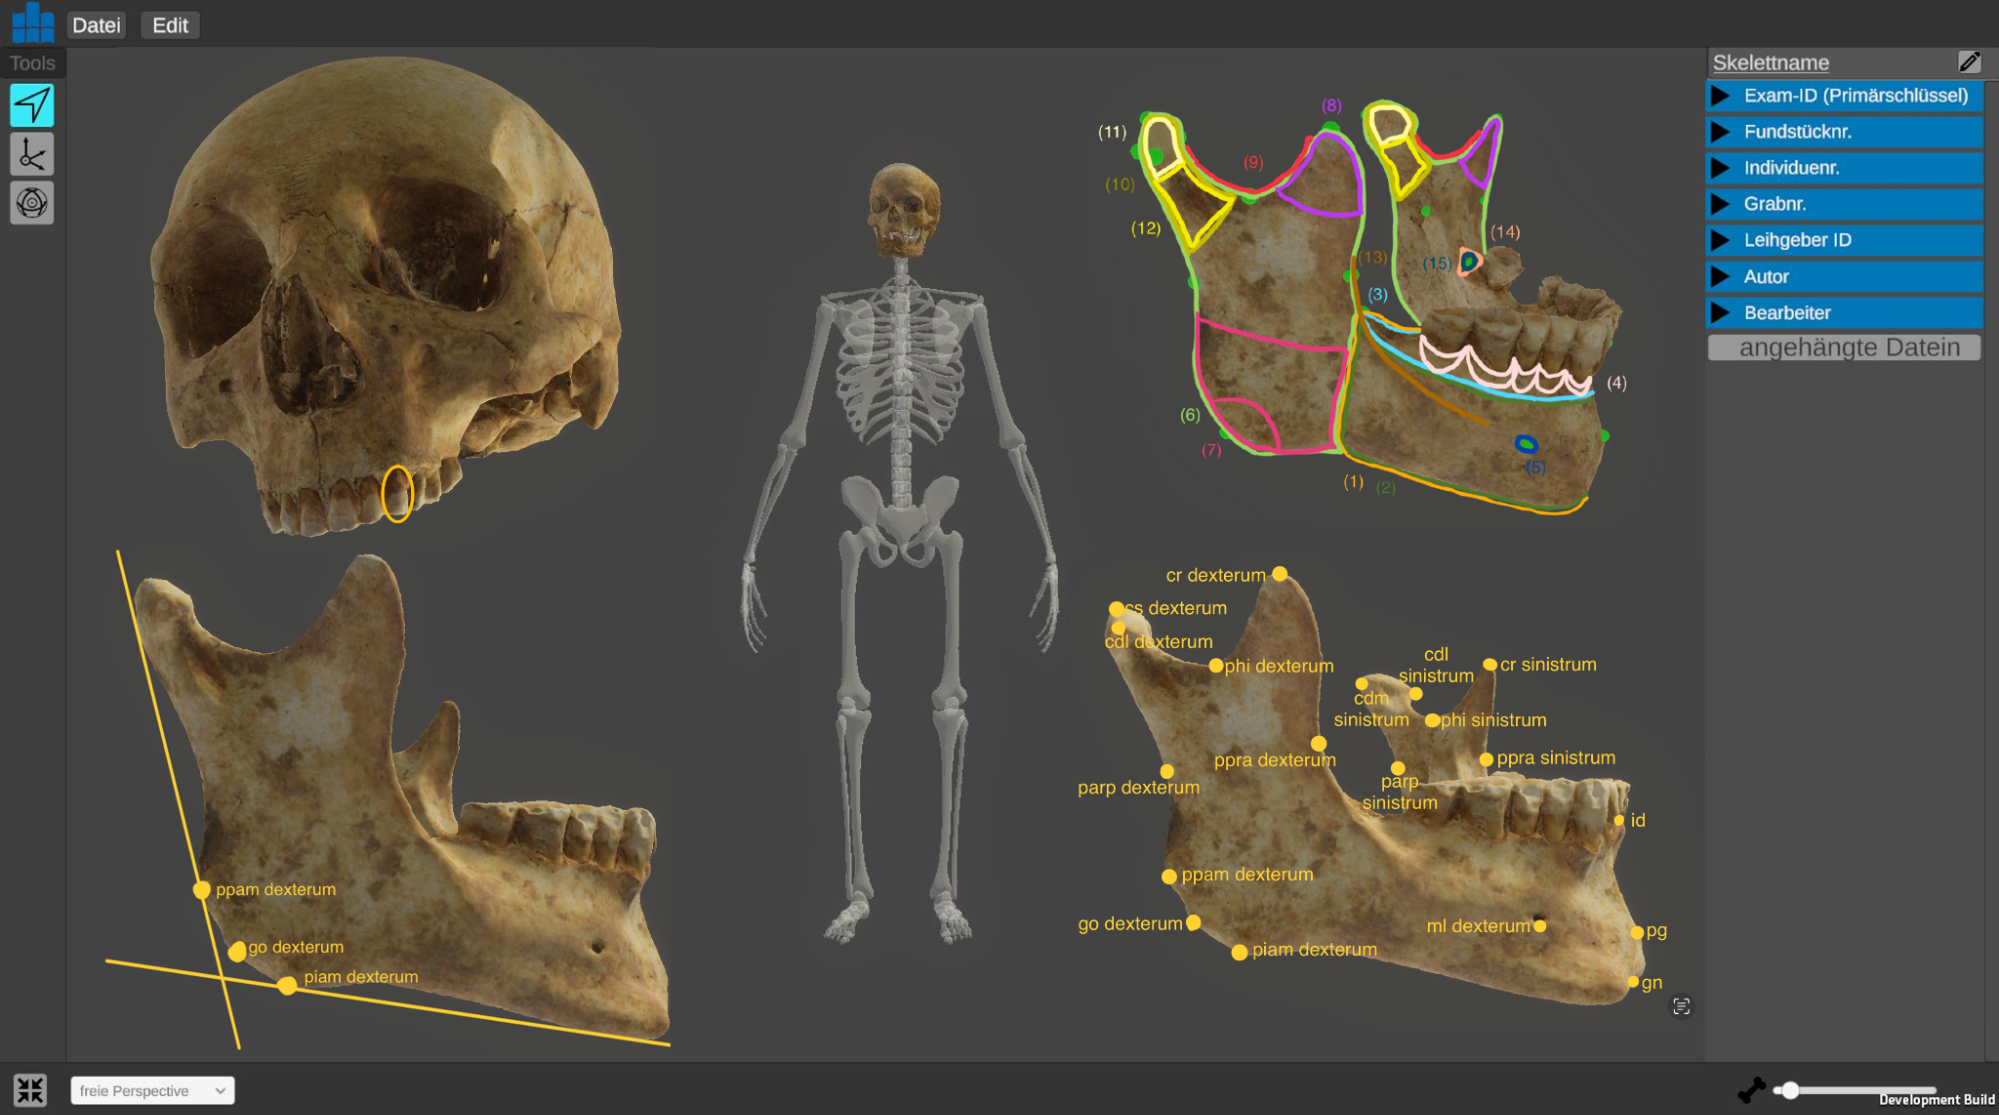
\includegraphics[width=\textwidth]{img/aw3d.png}
%\caption{3D model of a Cranium (skull) inserted into a placeholder skeleton in \aw{} depicting examples of various ANNOdc classes.}
\caption{
Collage of different views in \aw{} of a 3D model of a \emph{cranium} (skull) inserted into a placeholder skeleton (source:~\cite{aw3dcidoc}).
The cranium is a bone compound consisting of 29 bone elements.
One of them, the \emph{mandibula} (mandible), is flexibly connected to the rest of the skull by the mandibular joint.
In the top right, various bone parts on the Mandibula are visually emphasised, with part 14 representing the angulus mandibulae (mandibular angle).
In the top left, the \emph{dens caninus maxillaris dexter} (right maxillary secondary canine tooth), a tooth structure, is highlighted within a circle.
The tooth cusp is a part of the tooth.
It refers to the projection that divides the occlusal surface of most of the teeth, with the exception of the incisors.
At the bottom right, anatomical points (osteometric landmarks) of the right lateral side of the \emph{mandibula} are depicted.
The \emph{gonion dextrum} (right gonion; \emph{gonion dextrum}, abbreviated as \emph{go dextrum}, depicted alternative spelling of dextrum: dexterum) forms part of an anatomical line measuring the \emph{angulus mandibulae},
as shown in the bottom left.
Skeletal material courtesy of Dr. Birgit Grosskopf, Department of Historical Anthropology and Human Ecology, University of Göttingen.
}
\label{fig:aw3d}
\end{figure}

\begin{figure}[h]
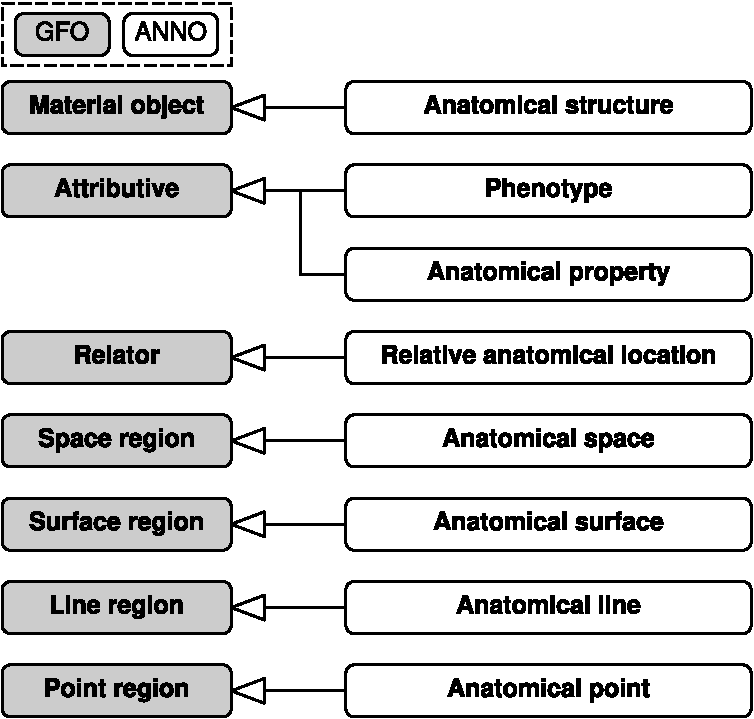
\includegraphics[width=0.6\textwidth]{img/gfo.pdf}
\caption{Integration of ANNO with the top-level GFO ontology.}\label{fig:gfo}
\end{figure}

\section{Development of ANNOds}\label{sec:domain}
% Arbeit der Domänenexperten, Tabelle, OWL-Generator
\begin{figure}[h!t]
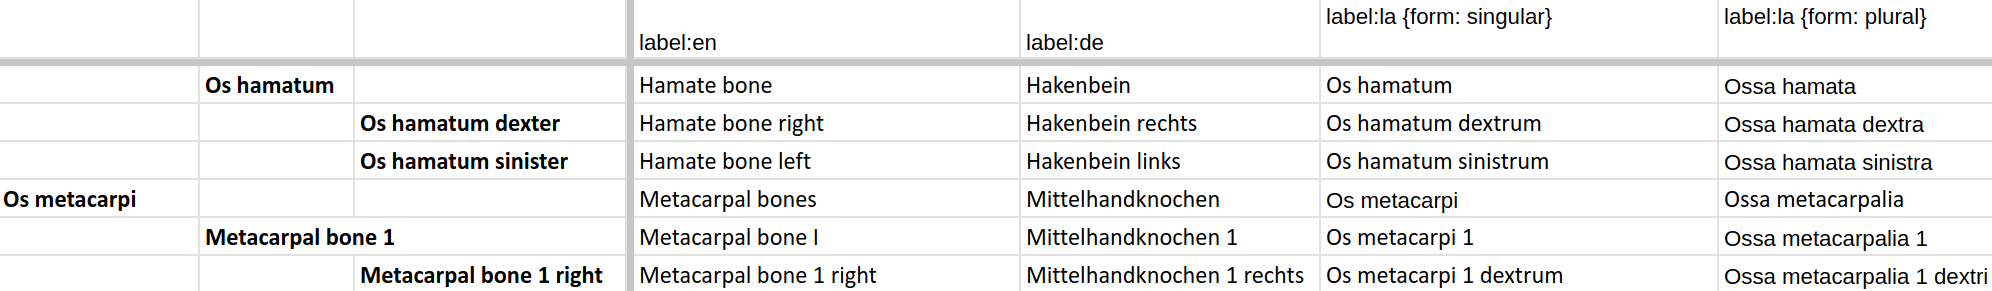
\includegraphics[width=\textwidth]{img/smog.png}
\caption{Excerpt of the spreadsheet-based input template used by the anthropologists.}\label{fig:smog}
\end{figure}


\section{Use Case: Integration into \aw{}}\label{sec:aw}

%\subsection{}\label{s1.1}
~\citep{rickview}
\section{Conclusion and Future Work}

%\begin{figure}[t]
%\includegraphics{}
%\caption{Figure caption.}\label{f1}
%\end{figure}

%\begin{table*}
%\caption{} \label{t1}
%\begin{tabular}{lll}
%\hline
%&&\\
%&&\\
%\hline
%\end{tabular}
%\end{table*}

\begin{ack}
\noindent\begin{minipage}{0.90\textwidth}
The ANNO project is co-financed from tax funds based on the budget passed by the Parliament of the Free State of Saxony.
\end{minipage}%
\hfill%
\begin{minipage}{0.04\textwidth}\raggedleft

\includegraphics[width=\textwidth]{img/saxony.pdf}
\end{minipage}
\end{ack}

\nocite{*}
\bibliographystyle{ios1}
\bibliography{paper}
\end{document}
